\documentclass{beamer}
\usetheme{Singapore}  % Choose the theme here
\usecolortheme{lily}  % Choose the color theme here
\usepackage{tikz} 
\usetikzlibrary{shapes,arrows,positioning}
\usepackage{graphicx} 
\usepackage{subcaption}
\usepackage{media9}
\usepackage{listings}
\usepackage{hyperref}
\usepackage{multimedia}

\lstset{
    language=Python,
    basicstyle=\ttfamily\small,
    backgroundcolor=\color{lightgray},
    numbers=left,
    numberstyle=\tiny,
    breaklines=true,
    captionpos=b
}
\bibliographystyle{plain} % Choose a bibliography style
\bibliography{ref}


% Title page information
\title{Choatic Systems: Solving the Lorenz Attractor with Recurrent Neural Network}
\author{Keran Chen}
\institute{University of Oslo}
\date{\today}

\AtBeginSection[]{
  \begin{frame}
    \vfill
    \centering
    \begin{beamercolorbox}[sep=8pt,center]{title}
      \usebeamerfont{title}\insertsectionhead\par%
    \end{beamercolorbox}
    \vfill
  \end{frame}
}

% Begin the document
\begin{document}

% Title slide
\begin{frame}
  \titlepage
\end{frame}

% Content slides

\begin{frame}[t]
	\frametitle{What's up: Some Motivations}
	\begin{itemize}
		\item Solving differential equations is important, but some are harder to solve than others. The lorenz attractor is such an case.
		\item Numerical methods might not always be accessible, e.g. when the exact form of the differential equation is not known. An alternative?
		\item We know that recurrent neural networks can solve differential equations, but how is it going to perform when it comes to a chaotic system?
	\end{itemize}
	
\end{frame}
\section{The Problem}

\begin{frame}[t]
	\frametitle{Stable Spiral}
	\begin{block}{Equation of Motion}
		
\begin{equation}
	\begin{aligned}
    \frac{dx}{dt} &= ax + by \notag,\\
    \frac{dy}{dt} &= cx + dy.
    \label{eq:spiral}
	\end{aligned}
\end{equation}
with $a = 0.2$, $b = -1.0$ , $c = 1.0$ , $d = 0.2$.	
\end{block}

\begin{block}{Characteristics}
	\begin{itemize}
		\item Converges to a fixed point
		\item Coupled
	\end{itemize}
\end{block}
\end{frame}
\begin{frame}
  \frametitle{Lorenz Attractor}
\begin{block}{Equation of motion}

\begin{equation}
\label{eq:lorenz}	
\begin{aligned}
\frac{{dx}}{{dt}} &= \sigma(y - x), \\
\frac{{dy}}{{dt}} &= x(\rho - z) - y, \\
\frac{{dz}}{{dt}} &= xy - \beta z,
\end{aligned}
\end{equation}	

with \(\sigma = 10\), \(\rho = 28\), and \(\beta = \frac{8}{3}\).
\end{block}
  \begin{block}{Characteristics of the Lorenz Attractor}
	  \begin{itemize}
		  \item Chaotic: sensitive to initial conditions
		  \item Coupled
	  \end{itemize}
  	
  \end{block}
\end{frame}

\section{The (Proposed) Solutions}
\begin{frame}
	\frametitle{Numerical Method}
	This is how we generate the data for training and testing!
	\begin{block}{Fourth Order Runge-Kutta (RK4)}
		\begin{itemize}
			\item Is not an exact solution
			\item Does not conserve energy
		\end{itemize}	
	\end{block}
\end{frame}

\begin{frame}[t]
	\frametitle{Recurrent Neural Network (RNN)}
	Unlike the Feed Forward Neural Network (FFNN), a Recurrent Neural Network can handle a time sequence. \\
	\begin{figure}[ht]
		\centering
		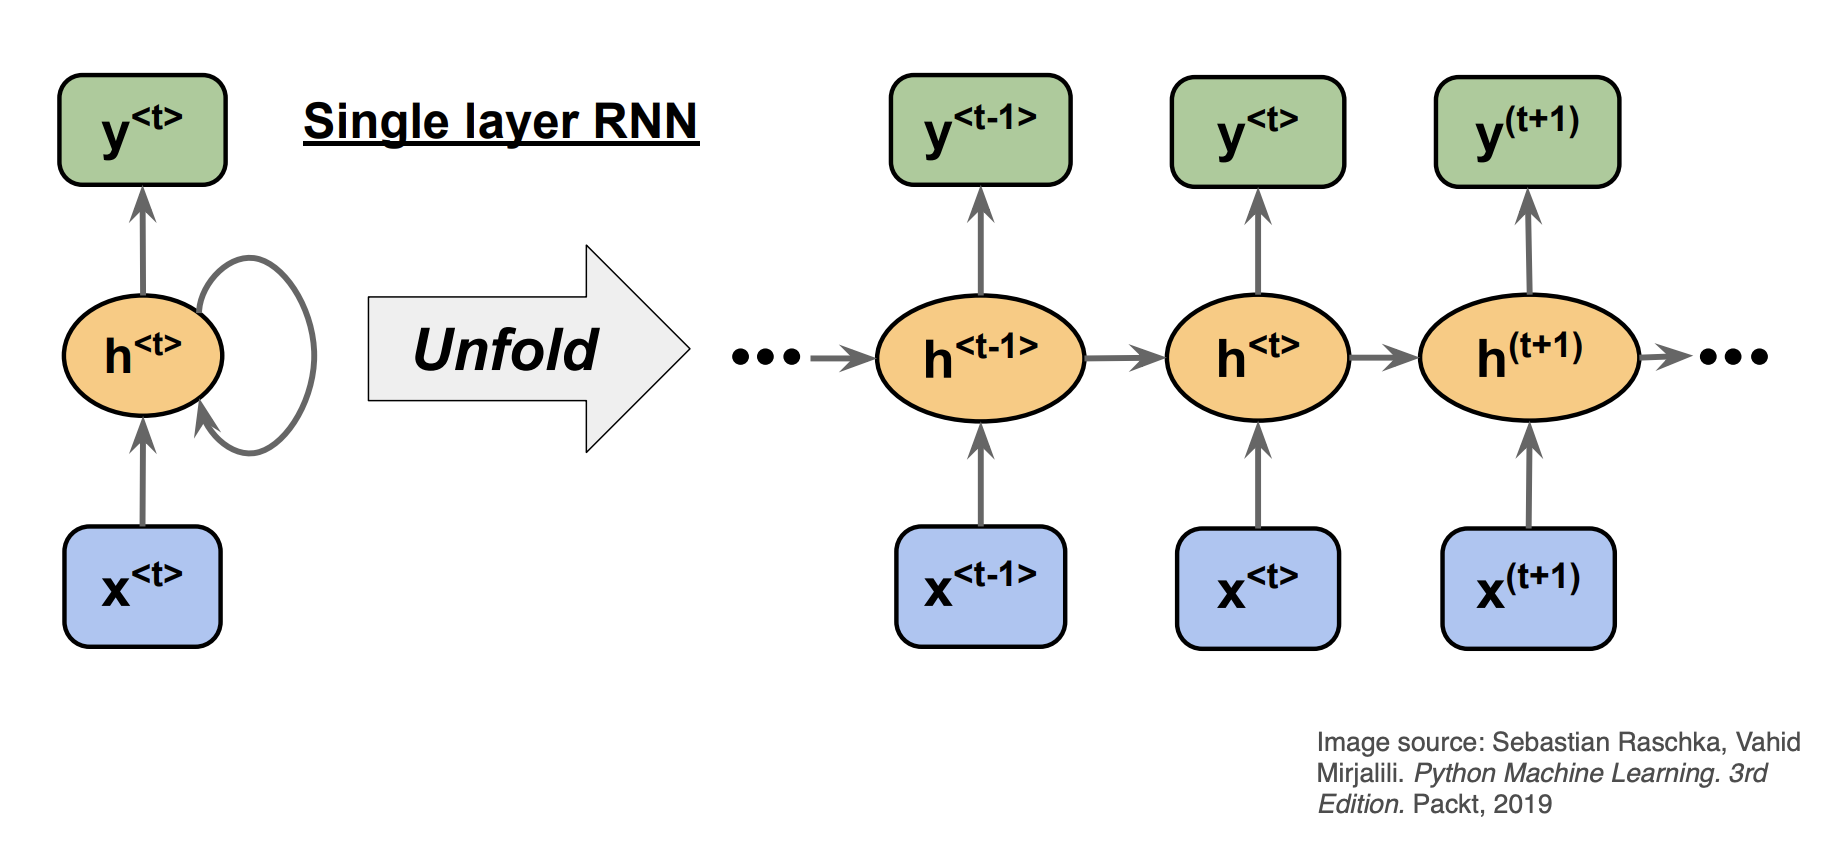
\includegraphics[width=0.8\textwidth]{images/RNN-pic.png}
	\end{figure}
\end{frame}

\begin{frame}[t]
	\frametitle{RNN}
	\begin{block}{Backpropagation through Time}
	The total loss $ L $ is
	\[L = \sum_{t=1}^T L^{(t)},\]
	and its derivative
	\[ \frac{\partial L^{(t)}}{\partial \boldsymbol{W}_{hh}} = \frac{\partial L^{(t)}}{\partial y^{(t)}}  \frac{\partial y^{(t)}}{\partial \boldsymbol{h}^{(t)}} 
	\left( \sum_{k=1}^{t} \frac{\partial \boldsymbol{h}^{(t)}}{\partial \boldsymbol{h}^{(k)}} \frac{\partial \boldsymbol{h}^{(k)}}{\partial \boldsymbol{W}_{hh}}  \right)   \] 
	\[ \frac{\partial \boldsymbol{h}^{(t)}}{\partial \boldsymbol{h}^{(k)}} = \prod_{i=k+1}^{t} \frac{\partial \boldsymbol{h}^{(i)}}{\partial \boldsymbol{h}^{(i-1)}}  \] 
	This product is the cause for the vanishing and exploding gradient.
	\end{block}
	How can we solve the problem of vanishing and exploding gradient? 
\end{frame}

\begin{frame}[t]
	\frametitle{Long Short Term Memory (LSTM)}
		
	\newcommand{\empt}[2]{$#1^{\langle #2 \rangle}$}

	\begin{figure}
	
	\begin{tikzpicture}[scale=0.95,
	    % GLOBAL CFG
	    font=\sf \scriptsize,
	    >=LaTeX,
	    % Styles
	    cell/.style={% For the main box
		rectangle, 
		rounded corners=5mm, 
		draw,
		very thick,
		},
	    operator/.style={%For operators like +  and  x
		circle,
		draw,
		inner sep=-0.5pt,
		minimum height =.2cm,
		},
	    function/.style={%For functions
		ellipse,
		draw,
		inner sep=1pt
		},
	    ct/.style={% For external inputs and outputs
		circle,
		draw,
		line width = .75pt,
		minimum width=1cm,
		inner sep=1pt,
		},
	    gt/.style={% For internal inputs
		rectangle,
		draw,
		minimum width=4mm,
		minimum height=3mm,
		inner sep=1pt
		},
	    mylabel/.style={% something new that I have learned
		font=\scriptsize\sffamily
		},
	    ArrowC1/.style={% Arrows with rounded corners
		rounded corners=.25cm,
		thick,
		},
	    ArrowC2/.style={% Arrows with big rounded corners
		rounded corners=.5cm,
		thick,
		},
	    ]

%Start drawing the thing...    
    % Draw the cell: 
	    \node [cell, minimum height =4cm, minimum width=6cm] at (0,0){} ;

	    % Draw inputs named ibox#
	    \node [gt] (ibox1) at (-2,-0.75) {$\sigma_f$};
	    \node [gt] (ibox2) at (-1.5,-0.75) {$\sigma_i$};
	    \node [gt, minimum width=1cm] (ibox3) at (-0.5,-0.75) {$\tanh_i$};
	    \node [gt] (ibox4) at (0.5,-0.75) {$\sigma_o$};

	   % Draw opérators   named mux# , add# and func#
	    \node [operator] (mux1) at (-2,1.5) {$\times$};
	    \node [operator] (add1) at (-0.5,1.5) {+};
	    \node [operator] (mux2) at (-0.5,0) {$\times$};
	    \node [operator] (mux3) at (1.5,0) {$\times$};
	    \node [function] (func1) at (1.5,0.75) {$\tanh_o$};

	    % Draw External inputs? named as basis c,h,x
	    \node[ct, label={[mylabel]Cell}] (c) at (-4,1.5) {\empt{c}{t-1}};
	    \node[ct, label={[mylabel]Hidden}] (h) at (-4,-1.5) {\empt{h}{t-1}};
	    \node[ct, label={[mylabel]left:Input}] (x) at (-2.5,-3) {\empt{x}{t}};

	    % Draw External outputs? named as basis c2,h2,x2
	    \node[ct, label={[mylabel]Next Cell}] (c2) at (4,1.5) {\empt{c}{t}};
	    \node[ct, label={[mylabel]Next Hidden}] (h2) at (4,-1.5) {\empt{h}{t}};
	    \node[ct, label={[mylabel]left:Output}] (x2) at (2.5,3) {\empt{h}{t}};

	% Start connecting all.
	    %Intersections and displacements are used. 
	    % Drawing arrows    
	    \draw [ArrowC1] (c) -- (mux1) -- (add1) -- (c2);

	    % Inputs
	    \draw [ArrowC2] (h) -| (ibox4);
	    \draw [ArrowC1] (h -| ibox1)++(-0.5,0) -| (ibox1); 
	    \draw [ArrowC1] (h -| ibox2)++(-0.5,0) -| (ibox2);
	    \draw [ArrowC1] (h -| ibox3)++(-0.5,0) -| (ibox3);
	    \draw [ArrowC1] (x) -- (x |- h)-| (ibox3);

	    % Internal
	    \draw [->, ArrowC2] (ibox1) -- (mux1);
	    \draw [->, ArrowC2] (ibox2) |- (mux2);
	    \draw [->, ArrowC2] (ibox3) -- (mux2);
	    \draw [->, ArrowC2] (ibox4) |- (mux3);
	    \draw [->, ArrowC2] (mux2) -- (add1);
	    \draw [->, ArrowC1] (add1 -| func1)++(-0.5,0) -| (func1);
	    \draw [->, ArrowC2] (func1) -- (mux3);

	    %Outputs
	    \draw [-, ArrowC2] (mux3) |- (h2);
	    \draw (c2 -| x2) ++(0,-0.1) coordinate (i1);
	    \draw [-, ArrowC2] (h2 -| x2)++(-0.5,0) -| (i1);
	    \draw [-, ArrowC2] (i1)++(0,0.2) -- (x2);

	\end{tikzpicture}

	\caption{LSTM illustration \footnote{source: https://tex.stackexchange.com/questions/432312/how-do-i-draw-an-lstm-cell-in-tikz}}
	\label{fig:lstm}
	\end{figure}

\end{frame}

\section{The Dataset}

\begin{frame}[t]
	\frametitle{RK4: Generation of Data}
	\framesubtitle{Lorenz Attractor}
	Produced result for 10 different particles each with 800 steps for 8 seconds. \\

	\begin{figure}
	    \centering
	    \begin{subfigure}[b]{0.45\textwidth}
	      \centering
	      \includegraphics[width=\textwidth]{images/p0-3d.pdf}
	      \caption{An example particle trajectories}
	      \label{fig:p03d}
	    \end{subfigure}
	    \hfill
	    \begin{subfigure}[b]{0.45\textwidth}
	      \centering
	      \includegraphics[width=\textwidth]{images/p0-xyz.pdf}
	      \caption{Components of the example trajectories}
	      \label{fig:p0-xyz}
	    \end{subfigure}
	  \end{figure}
	Treat these as the ``actual'' result and use the data for training and testing the neural networks. 
\end{frame}

\begin{frame}[t]
	\frametitle{RK4: Generation of Data}
	\framesubtitle{Spiral}
	Produced result for 10 different particles each with 800 steps for 8 seconds. \\

	\begin{figure}
	    \centering
	    \begin{subfigure}[b]{0.45\textwidth}
	      \centering
	      \includegraphics[width=\textwidth]{images/s0-2d.pdf}
	      \caption{An example particle trajectories}
	      \label{fig:p03d}
	    \end{subfigure}
	    \hfill
	    \begin{subfigure}[b]{0.45\textwidth}
	      \centering
	      \includegraphics[width=\textwidth]{images/s0-xy.pdf}
	      \caption{Components of the example trajectories}
	      \label{fig:p0-xyz}
	    \end{subfigure}
	  \end{figure}
	Treat these as the ``actual'' result and use the data for training and testing the neural networks. 
\end{frame}

\begin{frame}[t]
	\begin{center}
	\frametitle{Animation}
	\includemedia[
	    width=0.6\linewidth,
	    height=0.45\linewidth,
	    activate=pageopen,
	    addresource=images/p0-animation.mp4,
	    flashvars={
	      source=p0-animation.mp4
	    }
	  ]{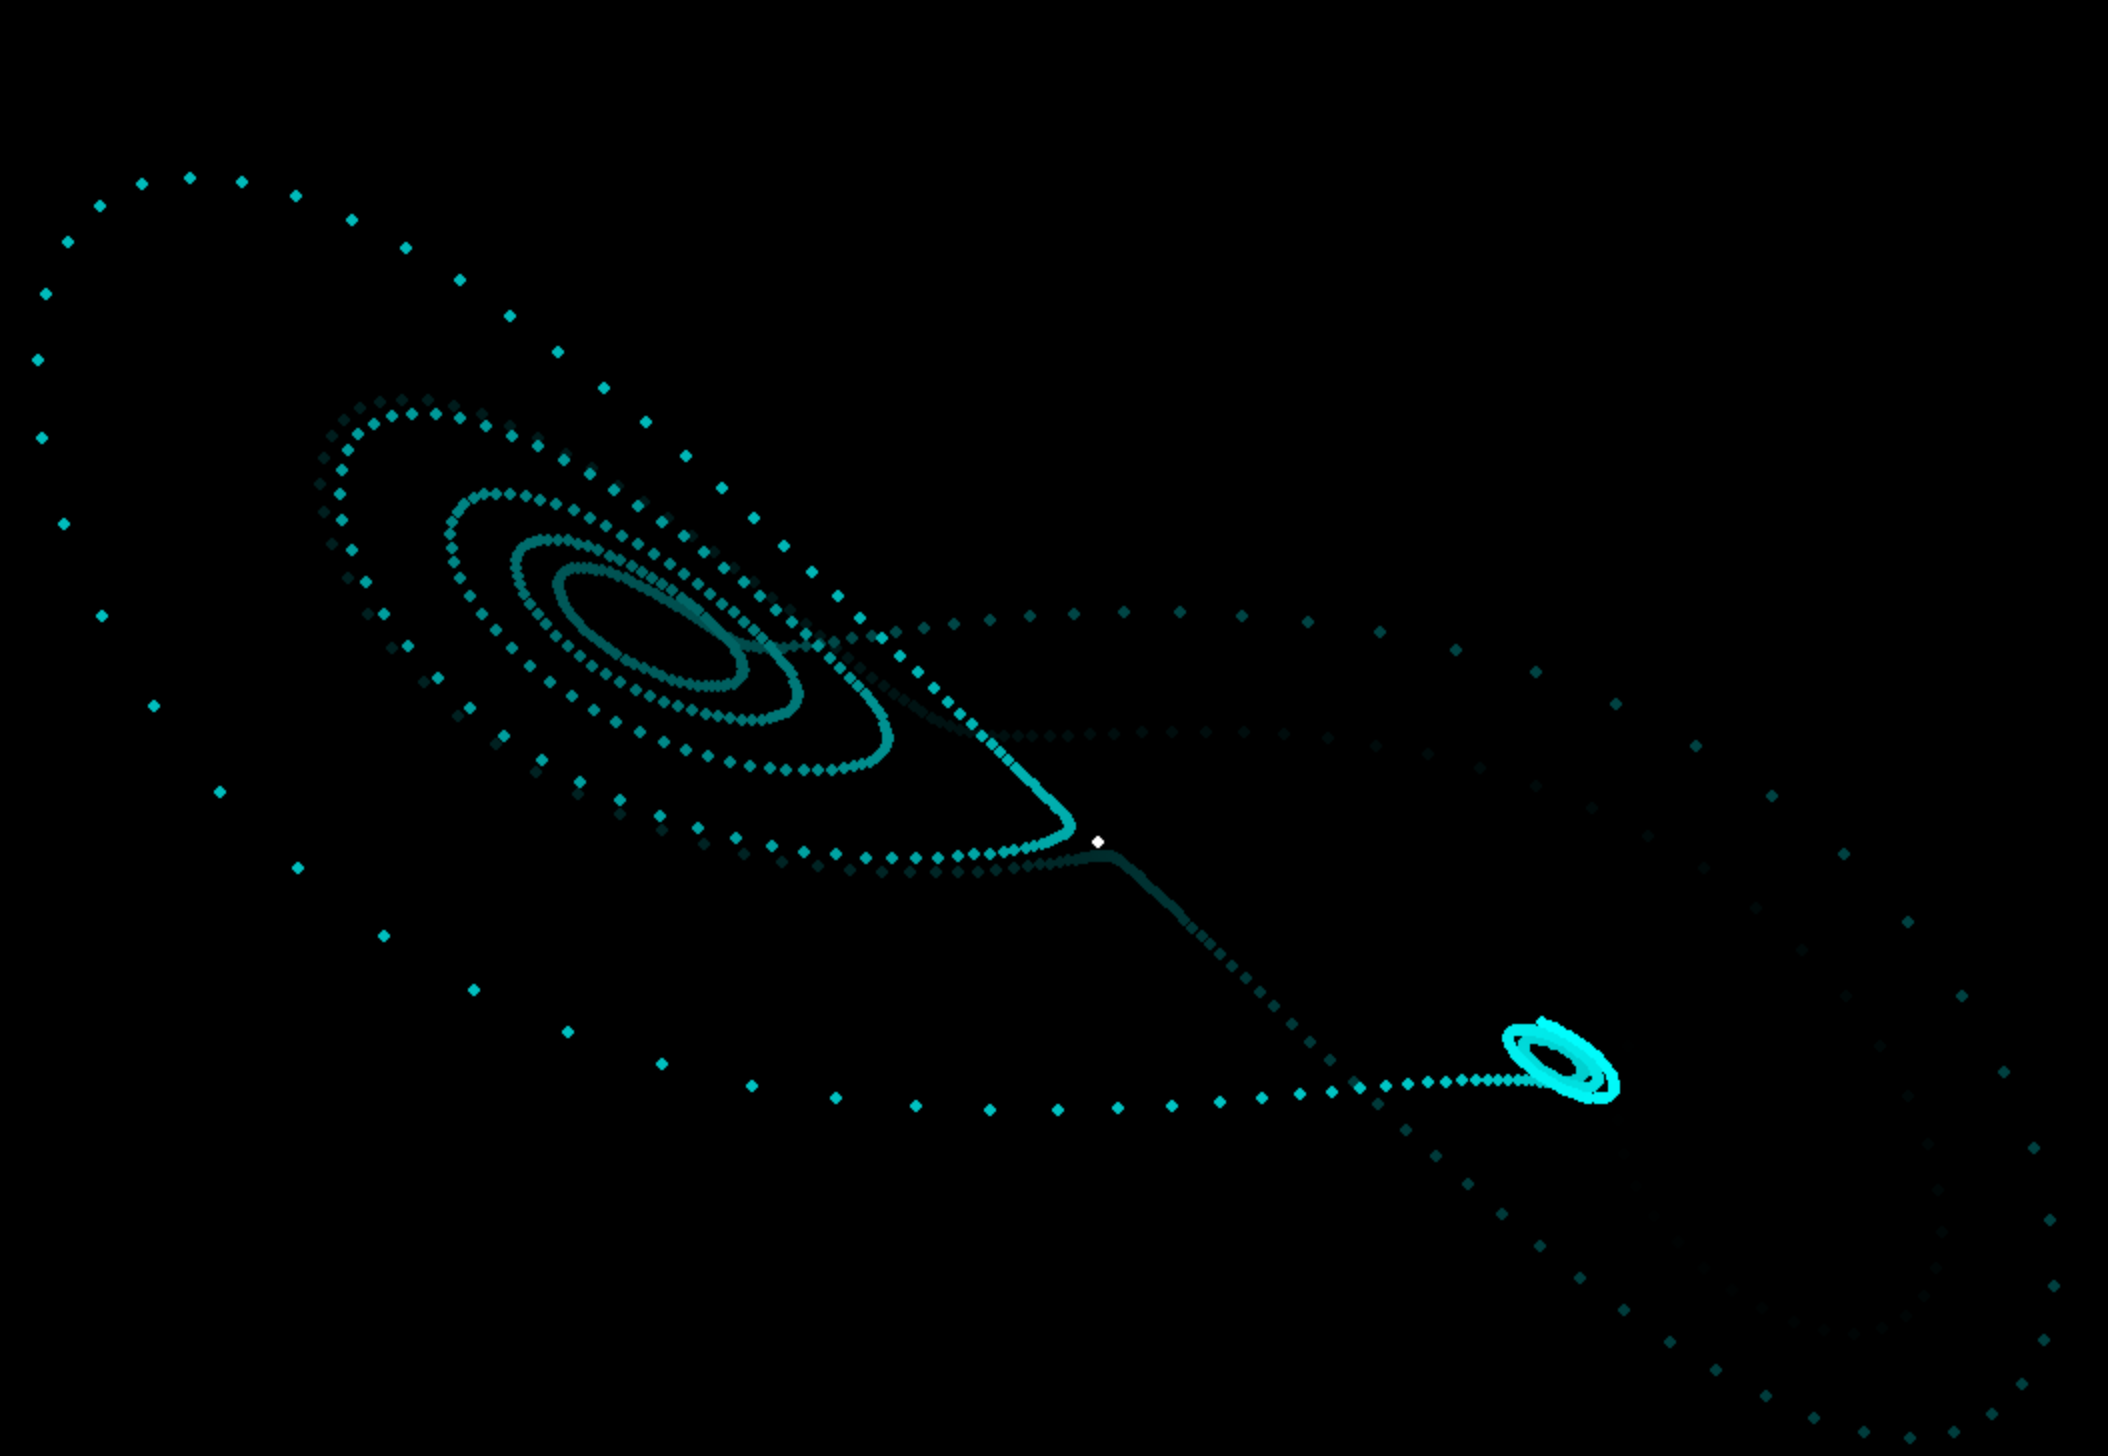
\includegraphics{images/place-holder.png}}{VPlayer.swf}
	  
	  \href{file:images/p0-animation.mp4}{Click here to play}
	  %url{file:Users/bukser/Desktop/UiO/Advance ML/final_pre_latex/images/p0-animation.mp4}
	  %\url{file:images/p0-animation.mp4}
  \end{center}
\end{frame}

\begin{frame}[t]
	\frametitle{Data Formatting}

	\begin{itemize}
		\item \texttt{train\_test\_split} $= 8:1 = 0.875$
		\item \texttt{input.shape} $ =(6384,$ \texttt{len\_seq}, \texttt{spatial\_dimension}). \\
		\item \texttt{target.shape} = (798,\texttt{spatial\_dimension})
	\end{itemize}
	For the Lorenz attractor \texttt{len\_seq} = 2 and \texttt{spatial\_dimension} = 3; for the stable spiral \texttt{len\_seq} = 2 and \texttt{spatial\_dimension} = 2 unless otherwise specified.

	
\end{frame}

\begin{frame}[t]
	\frametitle{The architecture}
	
We used functionalities from Tensorflow.keras to build our neural networks. \\
For both the vanilla RNN and LSTM, we used 
\begin{itemize}
	\item \texttt{n\_hidden} = 32, \texttt{n\_layers}=1
	\item optimizer: ADAM
	\item Loss function: MSE
\end{itemize}
\end{frame}

\section{The Results}

\begin{frame}[t]
	\frametitle{Neural Networks}
	\framesubtitle{FFNN}
	\begin{figure}[htpb]
		\centering
	      \includegraphics[scale=0.6]{images/lorenz_ffn_3d.pdf}
	      \caption{Predicted versus test trajectories for the FFNN on the Lorenz attractor}
	      \label{fig:ffnn-3d}
	\end{figure}
	
\end{frame}



\begin{frame}[t]
	\frametitle{Neural Networks}
	\framesubtitle{FFNN}
	{\color{red} Bad... } But why?

	\begin{figure}[ht]
		\centering
		\begin{subfigure}[b]{0.5\textwidth}
		\begin{center}
			\includegraphics[width=\textwidth]{images/lorenz_ffn.pdf}
		\end{center}
		\caption{Testing versus predicted trajectories decomposed by coordinates for the FFNN}
		\end{subfigure}
		\begin{subfigure}[b]{0.45\textwidth}
		      \centering
		      \includegraphics[width=\textwidth]{images/history_ffn.pdf}
		\caption{Normalised MAE of the FFNN for the prediction of Lorenz attractor}
		      \label{fig:history-ffn}
	    \end{subfigure}

		\caption{Prediction with FFNNs}
		\label{fig:ffnn}
	\end{figure}

	
\end{frame}

\begin{frame}[t]
	\frametitle{Neural Networks}
	\framesubtitle{FFNN}
	{\color{red} Bad...} But why?
	\begin{itemize}
		\item Overfitting
		\item Treats data point individually
	\end{itemize}
	
\end{frame}

\begin{frame}
  \frametitle{Neural Networks}
  \framesubtitle{RNNs: Spiral}
	\begin{columns}[T]
		
	\begin{column}{0.6\textwidth}
		
	\begin{figure}[ht]
		\centering
		      \centering
		      \includegraphics[width=\textwidth]{images/spiral_rnn.pdf}

		      \caption{Predicted versus test trajectories for the LSTM RNN on the Lorenz attractor}
		      \label{fig:spiral}

	\end{figure}
	\end{column}

	\begin{column}{0.35\textwidth}
		
	\begin{block}{MSE}
	\begin{itemize}
		\item Vanilla: 0.006
		\item LSTM: 0.005
	\end{itemize}
	\end{block}
	\end{column}

	\end{columns}
\end{frame}

\begin{frame}[t]
	\frametitle{Neural Networks}
	\framesubtitle{RNNs: Lorenz}
	\begin{figure}[ht]
		\centering
		\begin{subfigure}[b]{0.5\textwidth}
		\begin{center}
			\includegraphics[width=\textwidth]{images/lorenz_rnn.pdf}
		\end{center}
		\caption{Predictions for the Lorenz attractor trajectories with comparison for LSTM and Vanilla network.}
		\end{subfigure}
		\begin{subfigure}[b]{0.45\textwidth}
		      \centering
		      \includegraphics[width=\textwidth]{images/lorenz_rnn_lstm_vanilla_coordinates_errors.pdf}
		      \caption{Sum of the coordinate’s absolute errors for
the LSTM and Vanilla RNNs}
		      \label{fig:mae-rnn}
	    \end{subfigure}

		\label{fig:rnn}
	\end{figure}
	\begin{block}{MSE}
	Vanilla: 0.03	 $\quad$ LSTM: 0.02
	\end{block}

\end{frame}

\begin{frame}[t]
	\frametitle{Animations}	
	\begin{figure}[ht]
		\centering
	\movie[width=\textwidth, height=0.6\textheight, autostart, loop]
  {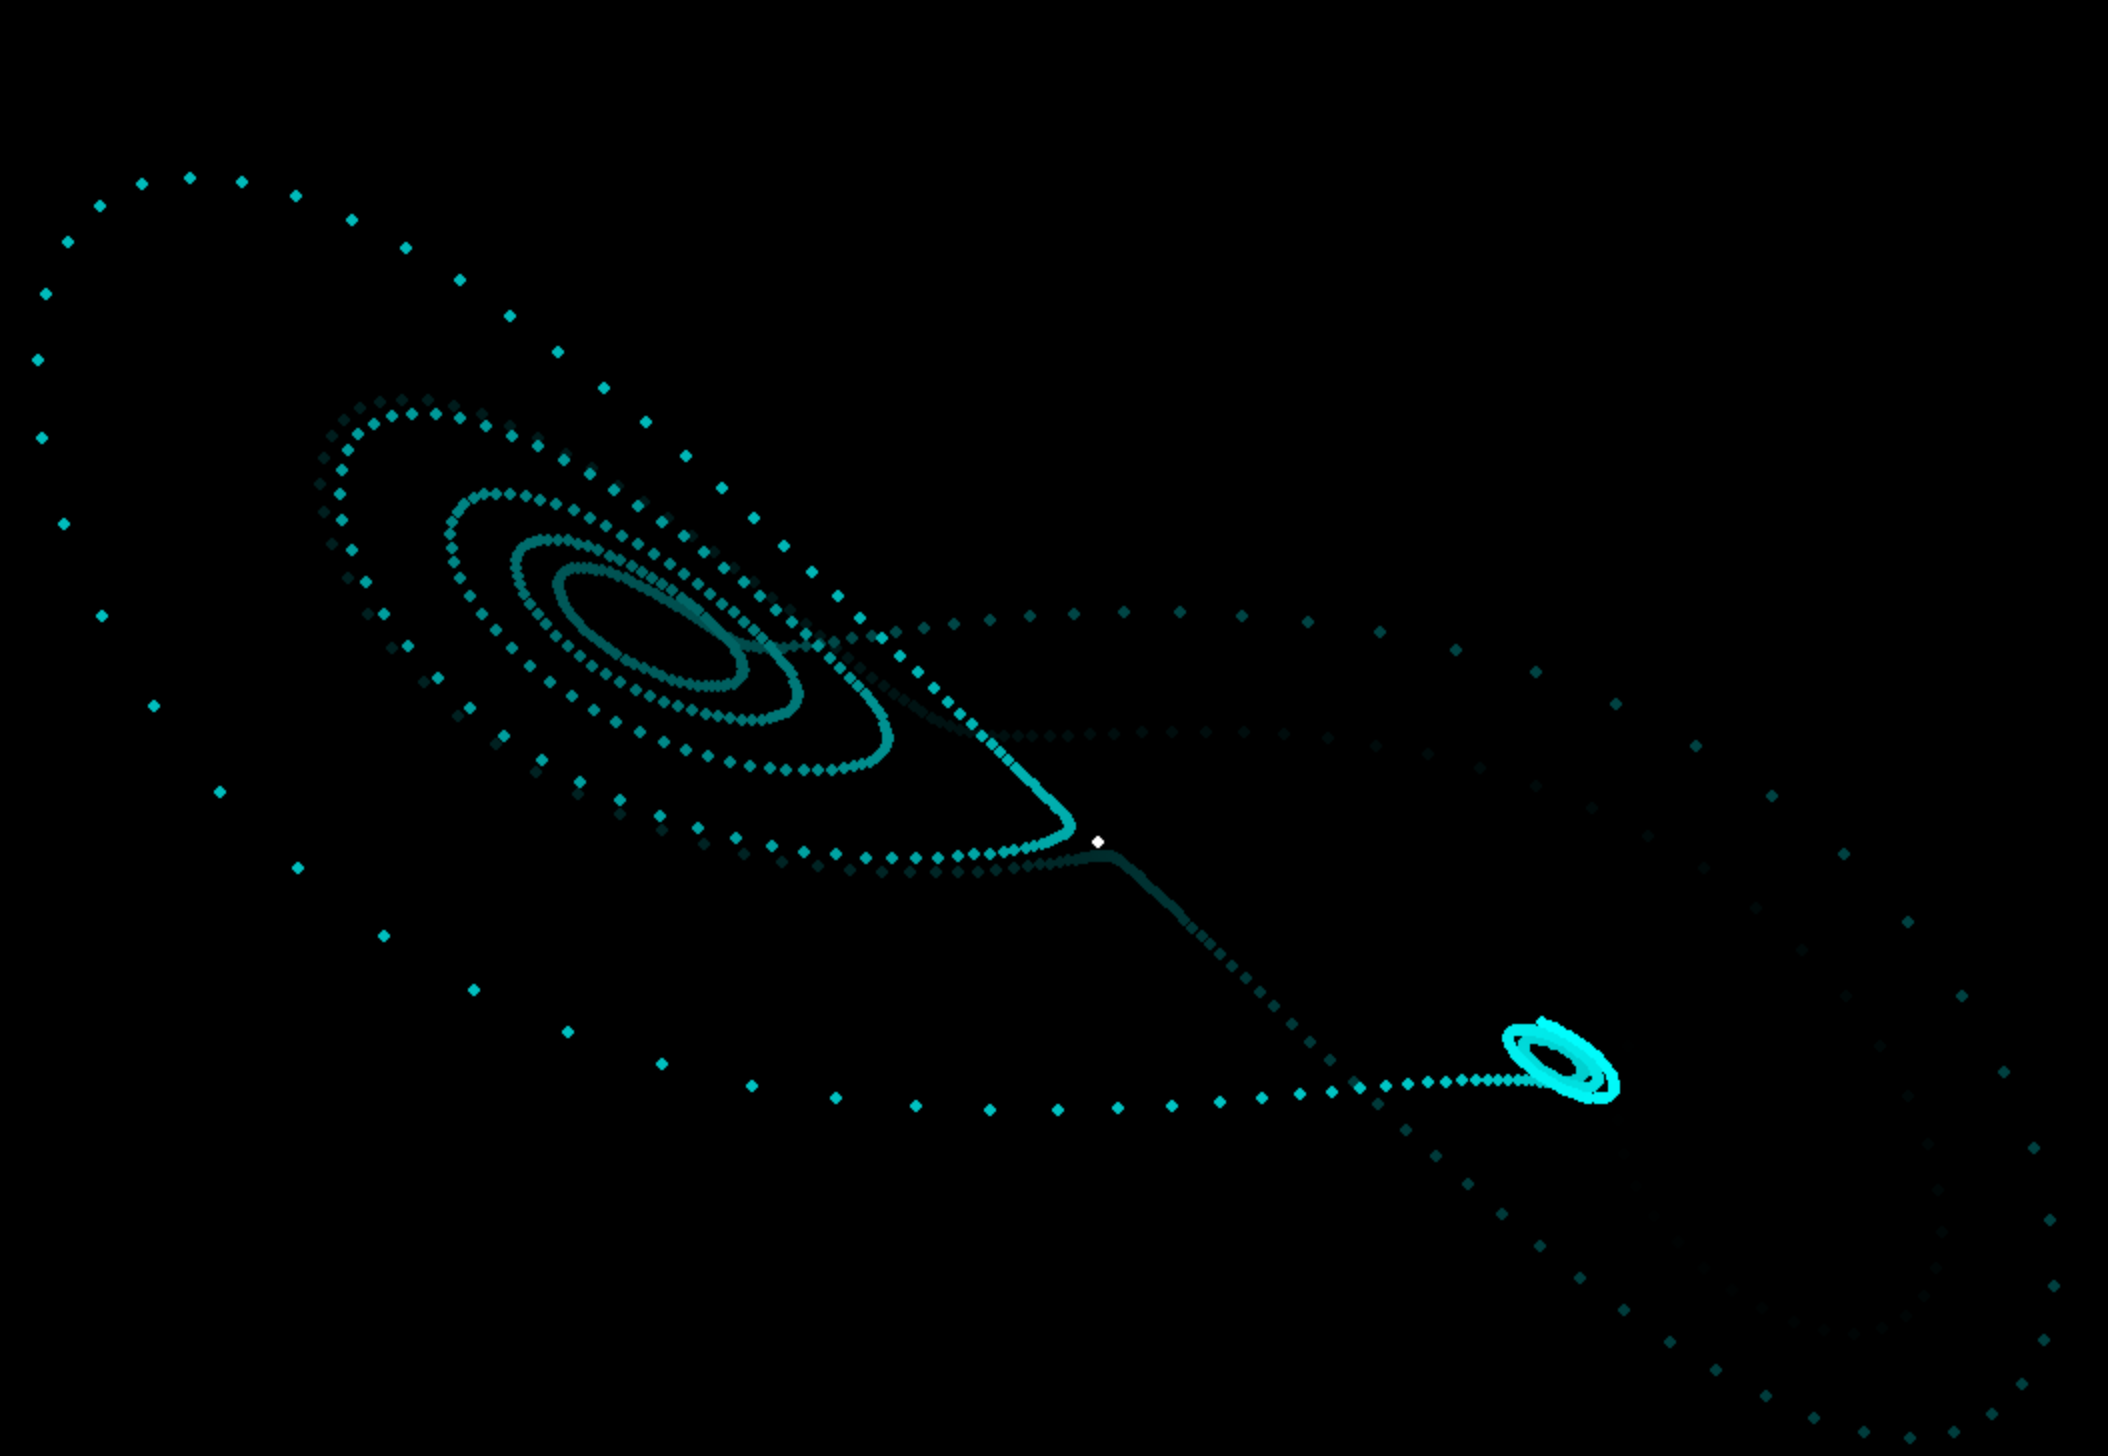
\includegraphics[width=\textwidth, height=0.6\textheight]{images/place-holder.png}}
  {images/lstm-xy.mp4}
	\end{figure}

	\begin{center}
		\href{file:images/lstm-xy.mp4}{lstm-xy}
		\hfill
		\href{file:images/lstm-yz.mp4}{lstm-yz}
		\hfill
		\href{file:images/vanilla-xy.mp4}{vanilla-xy}
	\end{center}
\end{frame}


\begin{frame}[t]
	\frametitle{RNNs: Hyperparameter Tuning}
	\framesubtitle{Lorenz}
	Basic grid search for hyperparameters: number of epochs, sequence length (look back).
	\begin{figure}[htpb]
		\centering
		\begin{subfigure}[b]{0.45\textwidth}
		      \centering
		      \includegraphics[width=\textwidth]{images/gridsearch_lenght_epochs_lstm.pdf}
		      \caption{Gridsearch of look-back and epochs for the LSTM trained on the Lorenz attractor trajectory.}
		      \label{fig:hp-lstm}
	    \end{subfigure}
		    \hfill
	    \begin{subfigure}[b]{0.45\textwidth}
		      \centering
		      \includegraphics[width=\textwidth]{images/gridsearch_lenght_epochs_vanilla.pdf}
		      \caption{Gridsearch of look-back and epochs for the vanilla RNN trained on the Lorenz attractor trajectory.}
		      \label{fig:hp-vanilla}
	    \end{subfigure}
	    \caption{Hyperparameter Tunning}
		\label{fig:grid}
	\end{figure}
\end{frame}

\begin{frame}[t]
	\frametitle{RNNs: Hyperparameter Tuning}
	\framesubtitle{Spiral}
	Basic grid search for hyperparameters: number of epochs, sequence length (look back).
	\begin{figure}[htpb]
		\centering
		\begin{subfigure}[b]{0.45\textwidth}
		      \centering
		      \includegraphics[width=\textwidth]{images/sprial_gridsearch_lenght_epochs_lstm.pdf}
		      \caption{Gridsearch of look-back and epochs for the LSTM trained on thespiral trajectory.}
		      \label{fig:hp-lstm-spiral}
	    \end{subfigure}
		    \hfill
	    \begin{subfigure}[b]{0.45\textwidth}
		      \centering
		      \includegraphics[width=\textwidth]{images/sprial_gridsearch_lenght_epochs_vanilla.pdf}
		      \caption{Gridsearch of look-back and epochs for the vanilla RNN trained on the spiral trajectory.}
		      \label{fig:hp-vanilla-spiral}
	    \end{subfigure}
	    \caption{Hyperparameter Tunning}
		\label{fig:grid-spiral}
	\end{figure}
	
\end{frame}




\begin{frame}[t]
	\frametitle{Physics Informed}
	To improve our network's performance, we tried changing the loss function so that the network respects the velocity (momentum) of the system.
	\[ \mathcal{L} = w_{MSE}\mathcal{L}_{MSE} + w_{PI}\mathcal{L}_{PI}. \] 
	We limited results to only $w_{MSE} = 1.0$ and $w_{PI}= 0.5$ 
	\begin{align}
    \mathcal{L}_{PI} &=     \frac{d \hat{x}}{dt} - \sigma (\hat{y}-\hat{x}) \notag\\
    & + \frac{d\hat{y}}{dt} - \hat{x}(\rho -\hat{z}) - \hat{y} \notag\\
    & +\frac{d\hat{z}}{dt} - \hat{x}\hat{y}- \beta \hat{z},
	\end{align}	
	where hats are used to denote the outputs of our networks.
\end{frame}
\begin{frame}[t]
	\frametitle{Physics Informed}
	In practice, we could not compute the derivatives effectively because our RNN predicts one times step at a time. So we did this instead:
	\begin{align}
	    \mathcal{L}_{PI} &=    MSE(\sigma (y-x), \sigma (\hat{y}-\hat{x})) \notag \\
	    & + MSE(x(\rho -z) - y , \hat{x}(\rho -\hat{z}) - \hat{y}) \notag \\
	    & +MSE(xy- \beta z , \hat{x}\hat{y}- \beta \hat{z})
	\end{align}
\end{frame}
\begin{frame}[t]
	\frametitle{Physics Informed}

	\begin{figure}[ht]
		\centering
		\begin{subfigure}[b]{0.5\textwidth}
		\begin{center}
			\includegraphics[width=\textwidth]{images/lorenz_rnn_lstm_lstmPI_coordinates_errors.pdf}
		\end{center}
		\caption{Sum of the absolute errors for all coordinates of the LSTM and physics-informed LSTM model for each time-step.}
		\end{subfigure}
		\begin{subfigure}[b]{0.45\textwidth}
		      \centering
		      \includegraphics[width=\textwidth]{images/lorenz_LSTMPI_rnn.pdf}

		      \caption{Comparing the predictions of Lorenz trajectories for the LSTM with and without an added physics-informed term to the loss function.}
		      \label{fig:rnn-pi}
	    \end{subfigure}

		\label{fig:PI}
	\end{figure}
So it's all good, right?
\end{frame}

\begin{frame}[t]
	\frametitle{Physics Informed?}
	Traditionally physics informed neural network uses appropriate choice of loss function in order to conserve some physical laws, such as conservation of energy, momentum or mass. ~\footnote{Karniadakis, G.E., Kevrekidis, I.G., Lu, L. et al. Physics-informed machine learning. Nat Rev Phys 3, 422–440 (2021). https://doi.org/10.1038/s42254-021-00314-5}\\
	We calculate the velocity by using the right hand side of Equation~\ref{eq:lorenz}, then compared with the velocity of the true values. \\
	{\color{red} The Lorenz Attractor does not have any conserved quantities. } 
	{\color{red} Is this actually adding any physics or are we just passing in more values for the same data point, i.e. both velocity and position?} 
\end{frame}

\begin{frame}[t]
	\frametitle{The Truths}
	\begin{itemize}
		\item Sometimes we see what we want to see.
		\item We didn't run it enough times to calculate the errors systematically but simply concluded that physics inform was indeed performing better than regular LSTM RNN.
		\item We weren't able to spot that the results for physics informed and LSTM are suspiciously similar... until yesterday.
	\end{itemize}
	\begin{block}{The Mistake}
	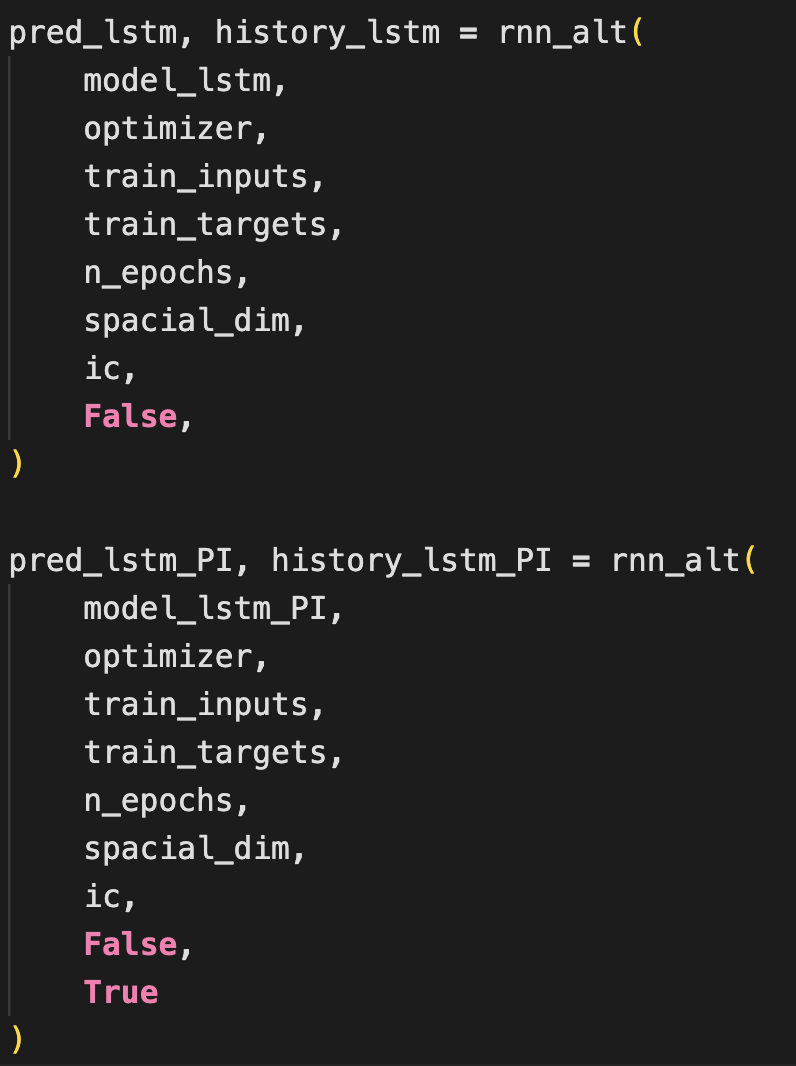
\includegraphics[width=0.3\linewidth]{images/mistake1.png}
	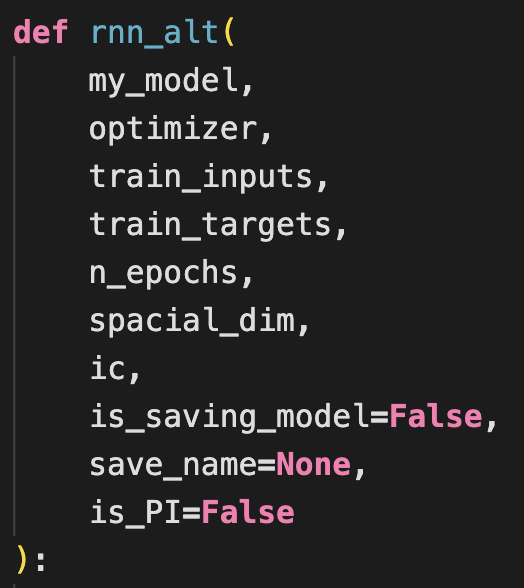
\includegraphics[width=0.3\linewidth]{images/mistake2.png}
	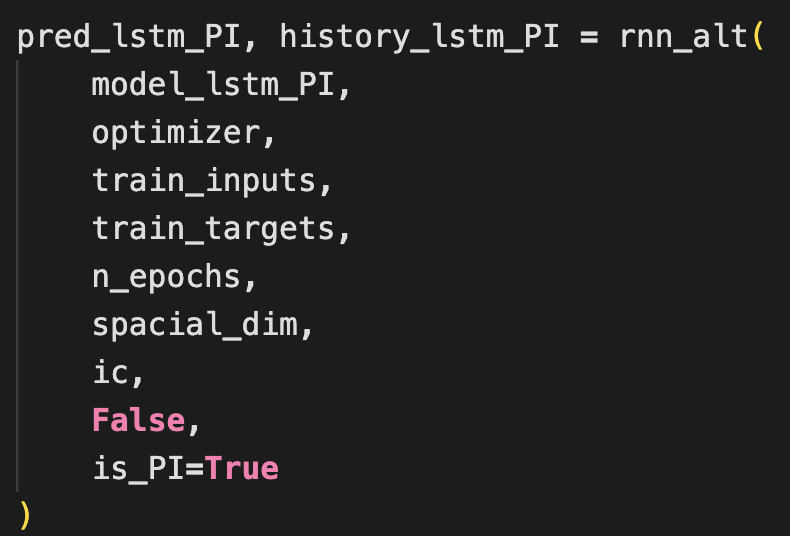
\includegraphics[width=0.35\linewidth]{images/mistake3.png}
	\end{block}
\end{frame}

\begin{frame}[t]
	\frametitle{The True Result}
	\begin{figure}[ht]
		\centering
		\begin{subfigure}[b]{0.5\textwidth}
		\begin{center}
			\includegraphics[width=\textwidth]{images/real-pi-traj.pdf}
		\end{center}
		\caption{Sum of the absolute errors for all coordinates of the LSTM and physics-informed LSTM model for each time-step.}
		\end{subfigure}
		\begin{subfigure}[b]{0.45\textwidth}
		      \centering
		      \includegraphics[width=\textwidth]{images/real-pi-errs.pdf}

		      \caption{Comparing the predictions of Lorenz trajectories for the LSTM with and without an added physics-informed term to the loss function.}
		      \label{fig:rnn-pi}
	    \end{subfigure}

		\caption{Prediction with RNNs}
		\label{fig:real-pi}
	\end{figure}
	
\end{frame}

\section{Conclusion}

\begin{frame}[t]
	\frametitle{Conclusion}
	\begin{itemize}
		\item FFNNs have underwhelming performances when it comes to time sequence, RNNs are much better suited to this task.
		\item Vanilla RNNs in general perform worse than LSTMs, for both the stable and chaotic case.
		\item The predictions for the stable spiral are in general superior to the Lorenz attractor, as expected.
		\item The best hyperparameters for the Vanilla RNN and the LSTM are number of epochs = 500 and look-back = 2.
		\item<2-> Always check your results!
	\end{itemize}
	
\end{frame}
\begin{frame}[t]
\frametitle{Future Work}
\begin{itemize}
\item Consider other types of RNNs, such as the Gated Recurrent Unit (GRU).
\item Explore other hyperparameters: number of hidden nodes etc.
\item Training on both the velocities and the positions
\item Predict the velocities as a vector field
\end{itemize}
\end{frame}


\begin{frame}[t]
\frametitle{Thank You}
\centering
Questions?
\end{frame}

\end{document}

